\documentclass[aspectratio=169,11pt]{beamer}
\usepackage[T1]{fontenc}
\usepackage[utf8]{inputenc}
\usepackage{lmodern}
\usepackage{array,booktabs}
\usepackage{listings}
\usepackage{tikz}
\usetikzlibrary{positioning,arrows.meta,fit,backgrounds,decorations.pathreplacing}

% Same TikZ styles as plan-style.sty, so the report's diagrams render unchanged.
\tikzset{box/.style={draw=black!65,rounded corners=3pt,minimum height=9mm,
 align=center,font=\small,inner sep=5pt},
 inputbox/.style={box,fill=blue!10},processbox/.style={box,fill=green!12},
 outputbox/.style={box,fill=orange!20},arrow/.style={-{Stealth[length=2mm]},thick},
 message/.style={arrow,dashed,draw=orange!85!black}}
\tikzset{card/.style={draw=black!25,fill=#1,rounded corners=4pt,minimum width=44mm,minimum height=30mm,align=center,inner sep=5pt}}
\newif\ifranktable % diagrams/header-details.tex: no rank table on the slides
\newcommand{\secnum}[1]{} % no report section numbers in the diagrams
\newcommand{\diagram}[1]{\resizebox{\linewidth}{!}{\input{diagrams/#1.tex}}}

\definecolor{navy}{HTML}{1B2340}
\definecolor{gold}{HTML}{D4A537}
\definecolor{cream}{HTML}{F6EDCF}
\setbeamercolor{frametitle}{fg=navy}
\setbeamercolor{title}{fg=navy}
\setbeamercolor{structure}{fg=navy}
\setbeamercolor{item}{fg=gold!85!black}
\setbeamerfont{frametitle}{series=\bfseries,size=\Large}
\setbeamertemplate{navigation symbols}{}
\setbeamertemplate{footline}{\hfill\scriptsize\color{black!50}
 DPHPC 2026 · Self-describing GOAL traces\quad\insertframenumber\hspace*{4mm}\vspace*{2mm}}
\setbeamertemplate{itemize items}[circle]

\lstset{basicstyle=\ttfamily\scriptsize,columns=fullflexible,keepspaces=true,
 breaklines=true,showstringspaces=false,frame=single,rulecolor=\color{black!18},
 backgroundcolor=\color{black!3},xleftmargin=3pt,xrightmargin=3pt}

% Shared encoding figures; the validation slide adds an overlay to the offset diagram.
\newcommand{\encodingfig}[1]{%
\begingroup
\def\encodingextra{#1}%
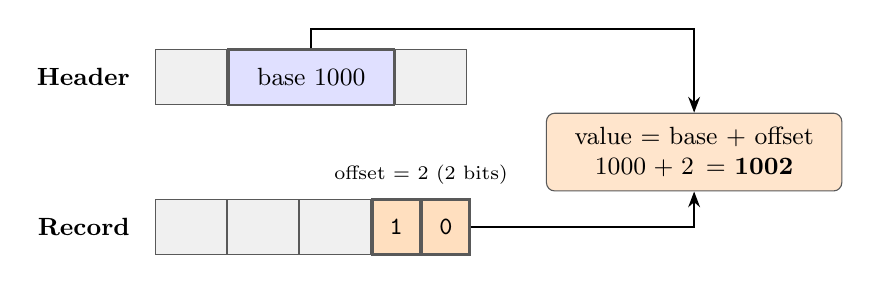
\begin{tikzpicture}[
  cell/.style={draw=black!65,minimum height=7mm,font=\small,inner sep=2pt},
  other/.style={cell,minimum width=9mm,fill=black!6},
  bit/.style={cell,minimum width=6mm,fill=orange!25,line width=0.9pt,font=\small\ttfamily}]
\node[font=\small\bfseries,anchor=east] at (-0.2,0) {Header};
\node[other,anchor=west] (h1) at (0,0) {};
\node[cell,fill=blue!12,line width=0.9pt,minimum width=21mm,right=0mm of h1] (base) {base 1000};
\node[other,right=0mm of base] (h2) {};
\node[font=\small\bfseries,anchor=east] at (-0.2,-1.9) {Record};
\node[other,anchor=west] (r1) at (0,-1.9) {};
\node[other,right=0mm of r1] (r2) {};
\node[other,right=0mm of r2] (r3) {};
\node[bit,right=0mm of r3] (f1) {1};
\node[bit,right=0mm of f1] (f2) {0};
\node[font=\scriptsize,above=0.5mm of f1.north east] {offset = 2 (2 bits)};
\node[outputbox,text width=34mm,right=10mm of h2.east,yshift=-9.5mm] (value) {value = base + offset\\$1000 + 2 =$ \textbf{1002}};
\draw[arrow] (base.north) -- ++(0,2.5mm) -| (value.north);
\draw[arrow] (f2.east) -| (value.south);
% Optional annotation used by the validation slide.
\ifdefined\encodingextra\encodingextra\fi
\end{tikzpicture}
%
\endgroup}
\newcommand{\dictfig}{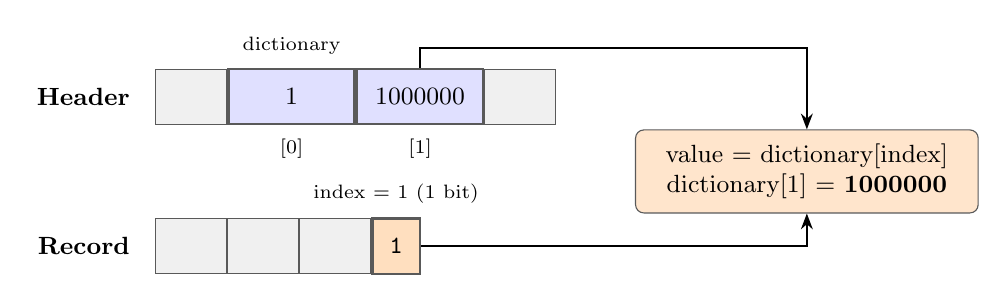
\begin{tikzpicture}[
  cell/.style={draw=black!65,minimum height=7mm,font=\small,inner sep=2pt},
  other/.style={cell,minimum width=9mm,fill=black!6},
  entry/.style={cell,minimum width=16mm,fill=blue!12,line width=0.9pt},
  bit/.style={cell,minimum width=6mm,fill=orange!25,line width=0.9pt,font=\small\ttfamily}]
\node[font=\small\bfseries,anchor=east] at (-0.2,0) {Header};
\node[other,anchor=west] (h1) at (0,0) {};
\node[entry,right=0mm of h1] (d0) {1};
\node[entry,right=0mm of d0] (d1) {1000000};
\node[other,right=0mm of d1] (h2) {};
\node[font=\scriptsize,below=0.5mm of d0] {[0]};
\node[font=\scriptsize,below=0.5mm of d1] {[1]};
\node[font=\scriptsize,above=0.5mm of d0] {dictionary};
\node[font=\small\bfseries,anchor=east] at (-0.2,-1.9) {Record};
\node[other,anchor=west] (r1) at (0,-1.9) {};
\node[other,right=0mm of r1] (r2) {};
\node[other,right=0mm of r2] (r3) {};
\node[bit,right=0mm of r3] (f1) {1};
\node[font=\scriptsize,above=0.5mm of f1.north] {index = 1 (1 bit)};
\node[outputbox,text width=40mm,right=10mm of h2.east,yshift=-9.5mm] (value) {value = dictionary[index]\\dictionary[1] = \textbf{1000000}};
\draw[arrow] (d1.north) -- ++(0,2.5mm) -| (value.north);
\draw[arrow] (f1.east) -| (value.south);
\end{tikzpicture}
}

% A row of example values for the encoding slides.
\newcommand{\vals}[1]{\foreach \v [count=\k] in {#1} \node[draw=black!65,fill=blue!8,minimum height=6mm,minimum width=14mm,font=\small,inner sep=2pt] at (\k*1.5,0) {\v};}

\newcolumntype{L}[1]{>{\raggedright\arraybackslash}p{#1}}
\newcommand{\smallnote}[1]{\par\vspace{2mm}{\small\color{black!60}#1}}
\newcommand{\highlight}[1]{\colorbox{cream}{\parbox{\dimexpr\linewidth-2\fboxsep}{\small #1}}}

\tikzset{runnercard/.style={draw=black!35,fill=#1,rounded corners=3pt,text width=44mm,align=left,
  inner sep=2.5mm,minimum height=27mm,anchor=north}}
% Contents of a runner card: name, role, how it decodes, strength, weakness.
\newcommand{\runner}[5]{%
  \scriptsize{\usebeamercolor[fg]{title}{\footnotesize\bfseries\ttfamily #1}}\\
  {\itshape\color{black!65}#2}\\[1.5mm]
  #3\\[1.5mm]
  {\color{green!45!black}$+$} #4\\
  {\color{red!60!black}$-$} #5\par}
\title{Self-describing GOAL traces for LogGOPSim}
\subtitle{DPHPC 2026 progress presentation}
\author{Joshua Durrant, Alexander Falter, Samuel Garcin, Mykhaylo Gershman}
\date{Supervised by Timo Schneider \\ 17.11.26}

\begin{document}

\begin{frame}
\titlepage
\end{frame}

\begin{frame}{Outline}
\begin{enumerate}
\item \textbf{Task:} the problem, our goals, who did what, structure of our implementation.
\item \textbf{Self-describing format:} file layout, encodings, conversion.
\item \textbf{Parallel conversion:} the first pass on OpenMP threads.
\item \textbf{Reading and validation:} simulator adapters, errors before the simulation starts.
\item \textbf{Case study: ATLAHS:} explicit GPU and message fields, two scheduler fixes.
\item \textbf{Fast decoding:} why it matters, one decode plan, five runners.
\item \textbf{Benchmarks:} writing (file size and conversion), then reading (all runners, throughput and startup).
\item Next steps and questions.
\end{enumerate}
\end{frame}

\section{Task}

\begin{frame}
\centering\vfill
{\usebeamercolor[fg]{title}\Huge\bfseries Task\par}
\vspace{3mm}
{\small\color{black!60}problem $\cdot$ goals $\cdot$ who did what $\cdot$ structure\par}
\vfill
\end{frame}

\begin{frame}{The problem: a fixed 39-byte record}
\diagram{legacy-record}
\vspace{2mm}
\begin{itemize}
\item Every node uses every field at full width, whatever values actually occur.
\item There is no place for extra information, so producers reuse fields.
\item ATLAHS puts the GPU into \texttt{nic} and packs five message components into the tag.
\item The file doesn't record this: a wrong guess simulates silently with wrong results.
\end{itemize}
\end{frame}

\begin{frame}{Goals and status}
\small
\begin{tabular}{L{0.3\linewidth}L{0.42\linewidth}L{0.2\linewidth}}
\toprule
\textbf{Goal} & \textbf{Question} & \textbf{Status} \\
\midrule
Self-describing, extensible traces & Can the file describe compact fields and extra attributes? & done \\
Load-time schema validation & Does the file supply what the simulator needs? & done \\
Runtime specialization & Can decoding exploit the known schema? & done: five runners \\
Benchmarking & Smaller and faster than legacy? & preliminary results; full study upcoming \\
\bottomrule
\end{tabular}
\vspace{4mm}
\begin{itemize}
\item LogGOPSim and ATLAHS's htsim both read the new format through the same reader.
\item Legacy files remain readable; legacy output is still the default.
\end{itemize}
\end{frame}

\begin{frame}{Who did what}
\small
\begin{tabular}{L{0.25\linewidth}L{0.68\linewidth}}
\toprule
\textbf{Name} & \textbf{Work} \\
\midrule
Joshua Durrant & Full benchmarking study (upcoming) \\
Alexander Falter & OpenMP-parallel first conversion pass (parallel GOAL reader, mergeable statistics, \texttt{-{}-threads}), its differential tests and benchmark \\
Samuel Garcin & Decode replay benchmark, decode plan (optimized interpreter), C JIT with cache, in-process JIT with LLVM ORC, differential test against the generic decoder \\
Mykhaylo Gershman & Self-describing format and converter, bit packing (including 0-bit constant fields), custom fields, validating reader and simulator adapters, LogGOPSim restructuring, ATLAHS integration, runner architecture and registry, templated runners, test suite (GoogleTest, pytest), benchmark suite and profiler, report \\
\bottomrule
\end{tabular}
\end{frame}

\begin{frame}{Structure of our implementation}
\centering\vfill
\diagram{design-overview}
\vfill
\end{frame}

\section{Self-describing format}

\begin{frame}
\centering\vfill
{\usebeamercolor[fg]{title}\Huge\bfseries Self-describing format\par}
\vspace{4mm}
{\large Mykhaylo Gershman\par}
\vspace{3mm}
{\small\color{black!60}file layout $\cdot$ encodings $\cdot$ conversion\par}
\vfill
\end{frame}

\begin{frame}{The self-describing file}
\diagram{file-sections}
\vspace{2mm}
\begin{itemize}
\item Same components as the legacy file (rank table, records, dependency lists, roots), but records and indices use inferred widths.
\item New: a \textbf{schema header} that describes every field, so a reader needs no built-in knowledge of the layout.
\item All records in a file share one layout, so node $i$ of a rank is found directly at \texttt{rank\_start + i $\times$ record\_size}, without scanning.
\item A new magic number distinguishes it from legacy files, which remain readable.
\end{itemize}
\end{frame}

\begin{frame}{The header describes every field}
\centering\vfill
\resizebox{\linewidth}{!}{% Header and rank table in file order (middle row), with one field descriptor (top) and one
% rank-table entry (bottom) zoomed in. Values in the zoomed rows are an example.
% \ifranktable draws the rank table; the report sets it, the slides leave it out because the
% rank table works as in the legacy format.
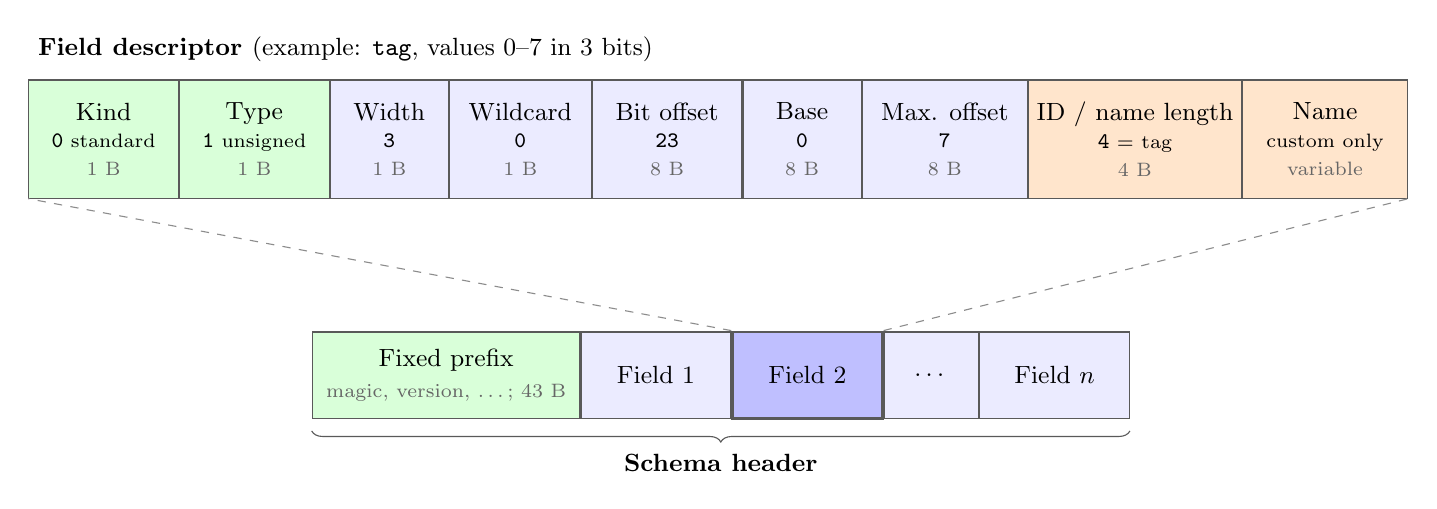
\begin{tikzpicture}[
  cell/.style={draw=black!65,minimum height=11mm,inner sep=1pt,align=center,font=\small},
  detail/.style={draw=black!65,minimum height=15mm,inner sep=1pt,align=center,font=\small},
  value/.style={font=\footnotesize\ttfamily},
  size/.style={font=\scriptsize\color{black!60}},
  zoom/.style={draw=black!45,dashed},
  part/.style={decorate,decoration={brace,amplitude=4pt},draw=black!65}]
% Middle row: the start of the file.
% Without the rank table, centre the header row under the enlarged descriptor.
\ifranktable\def\headerx{0mm}\else\def\headerx{36mm}\fi
\node[cell,fill=green!15,minimum width=34mm,anchor=west] (prefix) at (\headerx,0) {Fixed prefix\\{\scriptsize\color{black!60}magic, version, \dots; 43 B}};
\node[cell,fill=blue!8,minimum width=19mm,right=0mm of prefix] (f1) {Field 1};
\node[cell,fill=blue!25,line width=1pt,minimum width=19mm,right=0mm of f1] (f2) {Field 2};
\node[cell,fill=blue!8,minimum width=12mm,right=0mm of f2] (fd) {\dots};
\node[cell,fill=blue!8,minimum width=19mm,right=0mm of fd] (fn) {Field $n$};
\ifranktable
\node[cell,fill=black!6,minimum width=20mm,right=3mm of fn] (t0) {Rank 0};
\node[cell,fill=black!20,line width=1pt,minimum width=20mm,right=0mm of t0] (t1) {Rank 1};
\node[cell,fill=black!6,minimum width=12mm,right=0mm of t1] (td) {\dots};
\node[cell,fill=black!6,minimum width=20mm,right=0mm of td] (tr) {Rank $r{-}1$};
\draw[part] ([yshift=1.5mm]t0.north west) -- node[above=5pt,font=\small\bfseries] {Rank table} ([yshift=1.5mm]tr.north east);
\fi
% Each label sits on the side its zoom does not use.
\draw[part] ([yshift=-1.5mm]fn.south east) -- node[below=5pt,font=\small\bfseries] {Schema header} ([yshift=-1.5mm]prefix.south west);

% Top row: one field descriptor, 32 bytes plus the name of a custom field.
\begin{scope}[yshift=30mm]
\node[detail,fill=green!15,minimum width=19mm,anchor=west] (k) at (0,0) {Kind\\[-1pt]{\footnotesize\ttfamily 0}{\scriptsize\ standard}\\[-1pt]{\scriptsize\color{black!60}1 B}};
\node[detail,fill=green!15,minimum width=19mm,right=0mm of k] (ty) {Type\\[-1pt]{\footnotesize\ttfamily 1}{\scriptsize\ unsigned}\\[-1pt]{\scriptsize\color{black!60}1 B}};
\node[detail,fill=blue!8,minimum width=15mm,right=0mm of ty] (w) {Width\\[-1pt]{\footnotesize\ttfamily 3}\\[-1pt]{\scriptsize\color{black!60}1 B}};
\node[detail,fill=blue!8,minimum width=18mm,right=0mm of w] (wc) {Wildcard\\[-1pt]{\footnotesize\ttfamily 0}\\[-1pt]{\scriptsize\color{black!60}1 B}};
\node[detail,fill=blue!8,minimum width=19mm,right=0mm of wc] (bo) {Bit offset\\[-1pt]{\footnotesize\ttfamily 23}\\[-1pt]{\scriptsize\color{black!60}8 B}};
\node[detail,fill=blue!8,minimum width=15mm,right=0mm of bo] (b) {Base\\[-1pt]{\footnotesize\ttfamily 0}\\[-1pt]{\scriptsize\color{black!60}8 B}};
\node[detail,fill=blue!8,minimum width=21mm,right=0mm of b] (mo) {Max. offset\\[-1pt]{\footnotesize\ttfamily 7}\\[-1pt]{\scriptsize\color{black!60}8 B}};
\node[detail,fill=orange!20,minimum width=27mm,right=0mm of mo] (id) {ID / name length\\[-1pt]{\footnotesize\ttfamily 4}{\scriptsize\ = tag}\\[-1pt]{\scriptsize\color{black!60}4 B}};
\node[detail,fill=orange!20,minimum width=21mm,right=0mm of id] (nm) {Name\\[-1pt]{\scriptsize custom only}\\[-1pt]{\scriptsize\color{black!60}variable}};
\node[anchor=south west,font=\small\bfseries] at ([yshift=1mm]k.north west) {Field descriptor \normalfont(example: \texttt{tag}, values 0--7 in 3 bits)};
\end{scope}
\draw[zoom] (f2.north west) -- (k.south west);
\draw[zoom] (f2.north east) -- (nm.south east);

% Bottom row: one rank-table entry, 20 bytes.
\ifranktable
\begin{scope}[yshift=-30mm]
\node[detail,fill=orange!20,minimum width=60mm,anchor=west] (ro) at (20mm,0) {Start of rank data\\[-1pt]{\footnotesize byte \texttt{4096}}\\[-1pt]{\scriptsize\color{black!60}8 B}};
\node[detail,fill=black!6,minimum width=36mm,right=0mm of ro] (nc) {Node count\\[-1pt]{\footnotesize\ttfamily 7}\\[-1pt]{\scriptsize\color{black!60}4 B}};
\node[detail,fill=black!6,minimum width=36mm,right=0mm of nc] (dc) {Dependency count\\[-1pt]{\footnotesize\ttfamily 6}\\[-1pt]{\scriptsize\color{black!60}4 B}};
\node[detail,fill=black!6,minimum width=36mm,right=0mm of dc] (rc) {Root count\\[-1pt]{\footnotesize\ttfamily 1}\\[-1pt]{\scriptsize\color{black!60}4 B}};
\node[anchor=north west,font=\small\bfseries] at ([yshift=-1mm]ro.south west) {Rank-table entry \normalfont(example: rank 1)};
\end{scope}
\draw[zoom] (t1.south west) -- (ro.north west);
\draw[zoom] (t1.south east) -- (rc.north east);
\fi
\end{tikzpicture}
}
\vfill
\par\raggedright
\small
\begin{itemize}
\item Readers reject unknown versions and type codes, truncated headers and overlapping fields.
\end{itemize}
\end{frame}

\begin{frame}{Choosing an encoding for the fields}
\begin{itemize}
\item Each field already gets only as many bits as its largest value needs.
\item An \textbf{encoding} stores something smaller than the value itself, so it can save even more.
\end{itemize}
\vspace{4mm}
\textbf{Example 1:} one value repeated
\vspace{2mm}

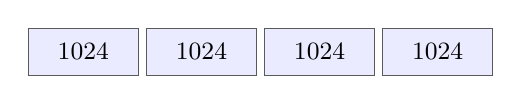
\begin{tikzpicture}[x=1cm]\vals{1024,1024,1024,1024}\end{tikzpicture}
\vspace{3mm}

Plain value: \textbf{11 bits} per value, although every value is the same.
\end{frame}

\begin{frame}{Offset encoding}
\begin{itemize}
\item The header stores the field's smallest value, the \textbf{base}; each record stores only the \textbf{offset} from it.
\end{itemize}
\vspace{4mm}
\centering\encodingfig{}
\par\raggedright
\vspace{4mm}
\begin{itemize}
\item Example 1: base 1024, every offset is 0, so \textbf{0 bits} per value instead of 11.
\end{itemize}
\end{frame}

\begin{frame}{A case offsets don't fix}
\textbf{Example 2:} two values far apart
\vspace{2mm}

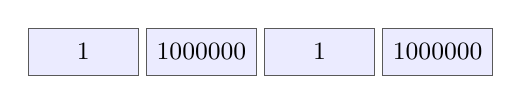
\begin{tikzpicture}[x=1cm]\vals{1,1000000,1,1000000}\end{tikzpicture}
\vspace{3mm}

\begin{itemize}
\item Plain value: \textbf{20 bits} per value, to hold 1,000,000.
\item Offset encoding: base 1, but offsets still reach 999,999, so still \textbf{20 bits}.
\end{itemize}
\end{frame}

\begin{frame}{Dictionary encoding (proposed)}
\begin{itemize}
\item The header stores the field's distinct values; each record stores only the \textbf{index} into that list.
\end{itemize}
\vspace{4mm}
\centering\dictfig
\par\raggedright
\vspace{4mm}
\begin{itemize}
\item Example 2: \textbf{1 bit} per value instead of 20, at the cost of storing the list in the header.
\end{itemize}
\end{frame}

\begin{frame}{Combining both}
\begin{itemize}
\item Offset encoding suits values close together; dictionary encoding suits few values far apart.
\item Using both, with the cheaper one chosen for each field, is probably the best approach.
\item Offset encoding is implemented; dictionary encoding and the combination are not yet.
\end{itemize}
\end{frame}

\begin{frame}{Conversion reads the input twice}
\diagram{conversion-overview}
\vspace{3mm}
\begin{itemize}
\item The layout must be fixed before the first record is written: if tags 0--7 fit in three bits but a later rank uses tag 1000, earlier records cannot be widened.
\item \textbf{Pass 1} keeps only file-wide statistics: each field's minimum and maximum, wildcards, dependency counts, the largest rank's node count.
\item \textbf{Pass 2} parses each rank again and packs its records, dependencies and roots with the final layout.
\item Each pass holds one rank's graph at a time, so memory is bounded by the largest rank and no temporary file is needed. The cost is parsing twice.
\end{itemize}
\end{frame}

\begin{frame}{Making conversion cheaper}
Reading and parsing the text twice costs time. Options we considered:
\vspace{3mm}

\footnotesize
\begin{tabular}{L{0.17\linewidth}L{0.29\linewidth}L{0.23\linewidth}L{0.23\linewidth}}
\toprule
\textbf{Idea} & \textbf{How} & \textbf{Trade-off} & \textbf{Status} \\
\midrule
Lighter first pass & Collect ranges and dependency counts without building the graph & Still reads the text twice & In progress: Alexander Falter, on the GPU \\
Temporary binary file & Parse once, store values in a temporary file, then pack from it & Extra disk space and I/O & Prototype: 1.36$\times$ faster on 2.1M nodes, 193 MB temporary data \\
Keep all graphs & Parse once and keep every rank in memory & Whole schedule must fit in memory & Infeasible for large schedules \\
Per-rank layouts & Choose a layout for each rank separately & One pass, but needs a format change & Proposed \\
\bottomrule
\end{tabular}
\vspace{4mm}

\highlight{\textbf{Switch by input size:} keep all graphs in memory when the schedule is small enough, otherwise fall back to a temporary file or two passes. Each option is then used where it is cheapest.}
\end{frame}

\begin{frame}[fragile]{Standard and custom fields}
\begin{columns}[T]
\begin{column}{0.44\textwidth}
\begin{lstlisting}
# config/custom_fields.toml
[[fields]]
name = "gpu_id"
type = "unsigned"
\end{lstlisting}
\begin{lstlisting}
l1: send 1024b to 1 tag 42 gpu_id 3
l2: calc 1000 gpu_id 3
\end{lstlisting}
\end{column}
\begin{column}{0.54\textwidth}
\begin{itemize}
\item \textbf{Custom fields} are declared in TOML and must appear on every operation.
\item From then on they're treated exactly like standard fields.
\item \textbf{Standard fields} (\texttt{type}, \texttt{peer}, \texttt{size}, \texttt{tag}, \texttt{cpu}, \texttt{nic}) stay standard because they're part of GOAL itself.
\item A file can contain fields a simulator doesn't need: each simulator reads only what it binds.
\end{itemize}
\end{column}
\end{columns}
\end{frame}

\section{Parallel conversion}

\begin{frame}
\centering\vfill
{\usebeamercolor[fg]{title}\Huge\bfseries Parallel conversion\par}
\vspace{4mm}
{\large Alexander Falter\par}
\vspace{3mm}
{\small\color{black!60}OpenMP first pass $\cdot$ same output as sequential $\cdot$ speedup\par}
\vfill
\end{frame}

\begin{frame}{Pass 1 in parallel: one rank per task}
{\centering\resizebox{0.78\linewidth}{!}{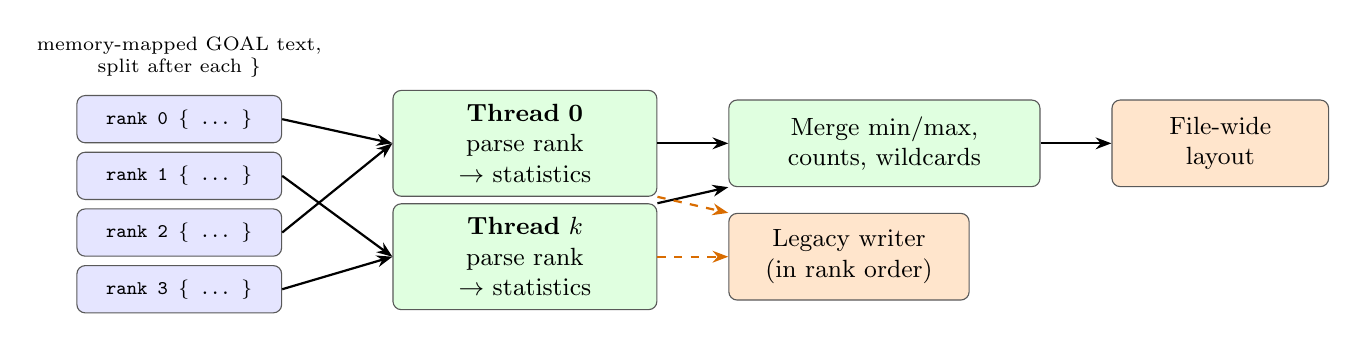
\begin{tikzpicture}[node distance=6mm and 9mm]
% The memory-mapped GOAL text, split after each rank block's closing brace.
\foreach \r/\y in {0/0,1/-1,2/-2,3/-3} {
  \node[inputbox,minimum width=26mm,minimum height=6mm,font=\scriptsize\ttfamily] (r\r) at (0,\y*0.72)
    {rank \r\ \{ \dots\ \}};
}
\node[font=\scriptsize,above=1mm of r0,align=center] {memory-mapped GOAL text,\\split after each \texttt{\}}};
% Threads parse whole ranks with the sequential scanner and keep their own statistics.
\node[processbox,text width=30mm,minimum height=11mm,right=14mm of r0.south east,anchor=west] (t0)
  {\textbf{Thread 0}\\parse rank $\to$ statistics};
\node[processbox,text width=30mm,minimum height=11mm,right=14mm of r2.south east,anchor=west] (t1)
  {\textbf{Thread $k$}\\parse rank $\to$ statistics};
\foreach \r/\t in {r0/t0,r1/t1,r2/t0,r3/t1} \draw[arrow] (\r.east)--(\t.west);
% Partial statistics are merged; legacy ranks are written in rank order.
\node[processbox,text width=36mm,minimum height=11mm,right=of t0] (m)
  {Merge min/max,\\counts, wildcards};
\node[outputbox,text width=24mm,minimum height=11mm,right=of m] (l) {File-wide\\layout};
\node[outputbox,text width=27mm,minimum height=11mm,right=of t1] (w)
  {Legacy writer\\(in rank order)};
\draw[arrow] (t0)--(m); \draw[arrow] (t1.north east)--(m.south west); \draw[arrow] (m)--(l);
\draw[message] (t0.south east)--(w.north west); \draw[message] (t1)--(w);
\end{tikzpicture}
}\par}
\vspace{1mm}
\footnotesize
\begin{itemize}
\item Ranks are independent in GOAL. The mapped input is cut after each rank's closing brace (not inside comments).
\item Each block is parsed by the unchanged re2c scanner, reading from memory instead of a \texttt{FILE*}.
\item Per-thread statistics: merging minima, maxima, counts and wildcard flags doesn't depend on order.
\item Legacy output is written in pass 1, so ranks reach the writer in rank order.
\end{itemize}
\end{frame}

\begin{frame}{Same result as the sequential pass}
\small
\begin{itemize}
\item \textbf{Identical output:} same bytes in both formats, same \texttt{-{}-report-schema} report.
\item \textbf{Identical errors:} if several ranks are invalid, the error of the lowest rank is reported, with the line number in the whole file and the same diagnostic text.
\item \textbf{Same limits:} one rank's graph per thread at a time; pipes fall back to the sequential reader. \texttt{txt2bin -{}-threads N} sets the thread count.
\item \textbf{One difference:} a second \texttt{num\_ranks} with a different value is rejected instead of applying to later ranks.
\end{itemize}
\vspace{2mm}
\highlight{\textbf{Tests:} 9 GoogleTest cases compare graphs, statistics and error messages with the sequential reader at 1, 2, 3 and 8 threads, in and out of rank order: CRLF, braces in comments, custom fields, syntax and structural errors.}
\end{frame}

\begin{frame}{Pass 1 speedup}
\small
Pass 1 alone (\texttt{first\_pass\_bench}): parse every rank and collect the statistics, \textbf{seconds}.
\vspace{2mm}

\centering
\footnotesize
\begin{tabular}{lrrrrrrr}
\toprule
\textbf{Trace} & \textbf{GOAL text} & \textbf{Sequential} & \textbf{1 thread} & \textbf{2} & \textbf{4} & \textbf{8} & \textbf{Speedup} \\
\midrule
dissemination\_65536 & 83 MB & 2.79 & 1.72 & 0.92 & 0.60 & 0.60 & \textbf{4.6$\times$} \\
allreduce\_ring\_2048 & 666 MB & 22.1 & 18.6 & 11.8 & 10.0 & 8.6 & \textbf{2.6$\times$} \\
alltoall\_4096 & 1.09 GB & 38.1 & 28.8 & 15.3 & 11.8 & 10.7 & \textbf{3.6$\times$} \\
\bottomrule
\end{tabular}
\par\raggedright\vspace{3mm}
\small
\begin{itemize}
\item Even on one thread the mapped reader is faster than the sequential \texttt{FILE*} reader.
\item Two threads nearly halve the time; beyond four threads it flattens. The cause is not measured yet.
\item Statistics are identical at every thread count (same hash of the report).
\end{itemize}
{\scriptsize\color{black!60}\par
Speedup: 8 threads against the sequential reader. Median of 3 runs, warm page cache, WSL2 with 8 vCPUs, g++-13 \texttt{-O2}. The machine was noisy: repeated runs of one configuration differed by up to 75\% (sequential reader on dissemination).}
\end{frame}

\begin{frame}{Complete conversion}
\small
Complete \texttt{txt2bin} run, \textbf{seconds}. Sequential: input through a pipe.
\vspace{2mm}

\centering
\footnotesize
\begin{tabular}{llrrrr}
\toprule
\textbf{Trace} & \textbf{Output} & \textbf{Sequential} & \textbf{1 thread} & \textbf{4 threads} & \textbf{8 threads} \\
\midrule
dissemination\_65536 & legacy & 1.60 & \textbf{1.18} & 2.95 & 5.37 \\
 & new format & n/a & 2.71 & & \textbf{1.86} \\
allreduce\_ring\_2048 & legacy & 14.9 & 13.7 & 7.7 & \textbf{6.7} \\
 & new format & n/a & 26.1 & & \textbf{20.0} \\
\bottomrule
\end{tabular}
\par\raggedright\vspace{3mm}
\small
\begin{itemize}
\item New format: 1.3--1.5$\times$ overall, since pass 2 is still sequential.
\item Legacy scales on ring (2.0$\times$) but not on dissemination: its 65,536 small ranks reach the writer one at a time.
\item The legacy writer now appends each rank instead of remapping the file: 2.79\,s $\to$ 1.18\,s on one thread.
\end{itemize}
{\scriptsize\color{black!60}\par
Median of 3--5 interleaved runs, same machine as before. n/a: the new format reads its input twice, so it can't come from a pipe.}
\end{frame}

\section{Reading and validation}

\begin{frame}
\centering\vfill
{\usebeamercolor[fg]{title}\Huge\bfseries Reading and validation\par}
\vspace{4mm}
{\large Mykhaylo Gershman\par}
\vspace{3mm}
{\small\color{black!60}simulator adapters $\cdot$ load-time checks $\cdot$ backward compatibility\par}
\vfill
\end{frame}

\begin{frame}{Reading: adapters bind fields to node structs}
\centering\resizebox{!}{0.5\textheight}{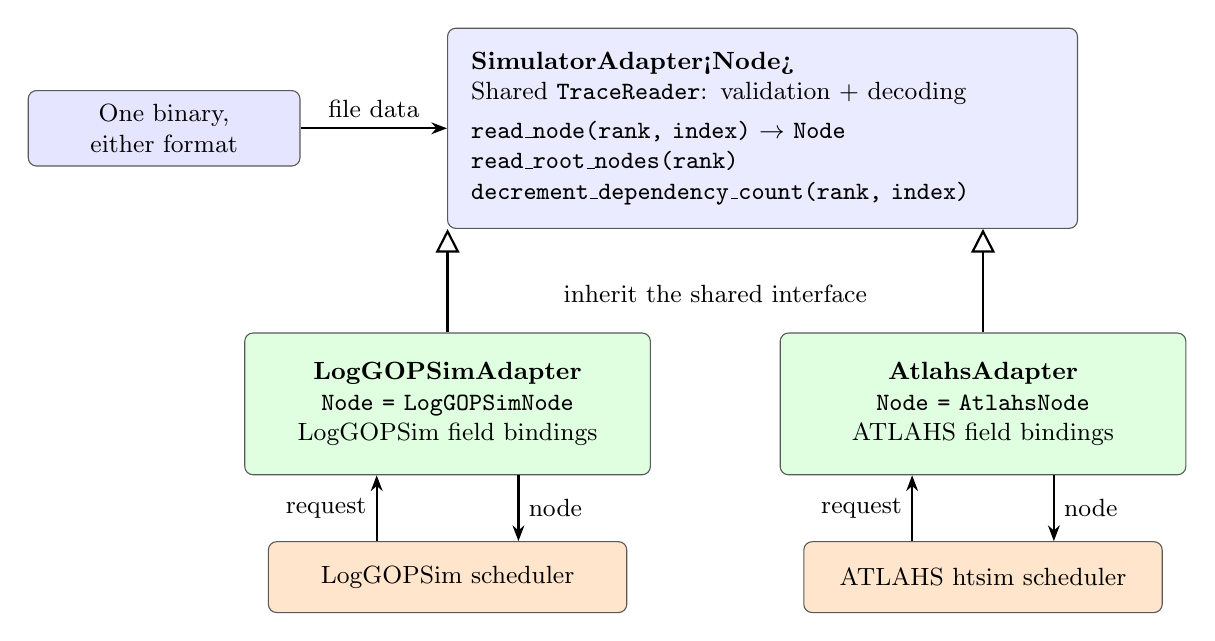
\begin{tikzpicture}[
  common/.style={box,fill=blue!8,text width=74mm,align=left,inner sep=3mm},
  adapter/.style={box,fill=green!12,text width=48mm,minimum height=18mm},
  inherits/.style={-{Triangle[open,length=3mm,width=3mm]},thick}]
\node[inputbox,text width=31mm] (file) at (0,0) {One binary,\\either format};
\node[common] (base) at (7.6,0) {
  \textbf{SimulatorAdapter<Node>}\\
  Shared \texttt{TraceReader}: validation + decoding\\[3pt]
  \texttt{read\_node(rank, index)} $\rightarrow$ \texttt{Node}\\
  \texttt{read\_root\_nodes(rank)}\\
  \texttt{decrement\_dependency\_count(rank, index)}};
\draw[arrow] (file) -- node[above,font=\small] {file data} (base);
\node[adapter] (log) at (3.6,-3.5) {\textbf{LogGOPSimAdapter}\\\texttt{Node = LogGOPSimNode}\\LogGOPSim field bindings};
\node[adapter] (atlas) at (10.4,-3.5) {\textbf{AtlahsAdapter}\\\texttt{Node = AtlahsNode}\\ATLAHS field bindings};
\draw[inherits] (log.north) -- (log.north |- base.south);
\draw[inherits] (atlas.north) -- (atlas.north |- base.south);
\node[font=\small,fill=white] at (7,-2.1) {inherit the shared interface};
\node[outputbox,text width=42mm] (ls) at (3.6,-5.7) {LogGOPSim scheduler};
\node[outputbox,text width=42mm] (as) at (10.4,-5.7) {ATLAHS htsim scheduler};
\draw[arrow] ([xshift=-9mm]ls.north) -- node[left,font=\small] {request} ([xshift=-9mm]log.south);
\draw[arrow] ([xshift=9mm]log.south) -- node[right,font=\small] {node} ([xshift=9mm]ls.north);
\draw[arrow] ([xshift=-9mm]as.north) -- node[left,font=\small] {request} ([xshift=-9mm]atlas.south);
\draw[arrow] ([xshift=9mm]atlas.south) -- node[right,font=\small] {node} ([xshift=9mm]as.north);
\end{tikzpicture}
}
\par\raggedright
\small
\begin{itemize}
\item Each simulator declares its node type and binds file fields to its members; unbound fields are skipped, so one file serves several simulators.
\item The file is memory-mapped; a node is decoded only when the scheduler requests it, and counters are decremented in a private copy, so the file can be reused.
\end{itemize}
\end{frame}

\begin{frame}{Validation: errors before the simulation starts}
\textbf{At load time}, the reader checks that every field the simulator needs exists and that its values fit the simulator's node struct, using only the header.
\vspace{6mm}

\centering
\resizebox{0.95\linewidth}{!}{\encodingfig{%
  \node[box,fill=red!12,text width=25mm,right=20mm of value] (member) {Node member\\\texttt{uint8\_t}: 0--255};
  \draw[arrow,red!70!black] (value) -- node[above,font=\scriptsize,align=center]{1000--1003\\don't fit} (member);}}
\par\raggedright
\vspace{3mm}

\small
Example: the file says the field holds 1000--1003, but the simulator stores it in a \texttt{uint8\_t}. Copying 1002 would silently give 234, so the reader refuses the file before reading any node.
\vspace{2mm}

\textbf{When a node is read}, cheap checks catch corrupt records (bounds, operation codes, peer ranks).
\vspace{3mm}

\highlight{A missing or incompatible field is a clear error, instead of a silently misread value.}
\end{frame}

\begin{frame}{Backward compatibility: one reader, both formats}
\vspace{2mm}\centering\resizebox{!}{0.42\textheight}{% Backward compatibility: one TraceReader picks the reader for the file's format; both take the
% adapter's field bindings and fill the same node struct.
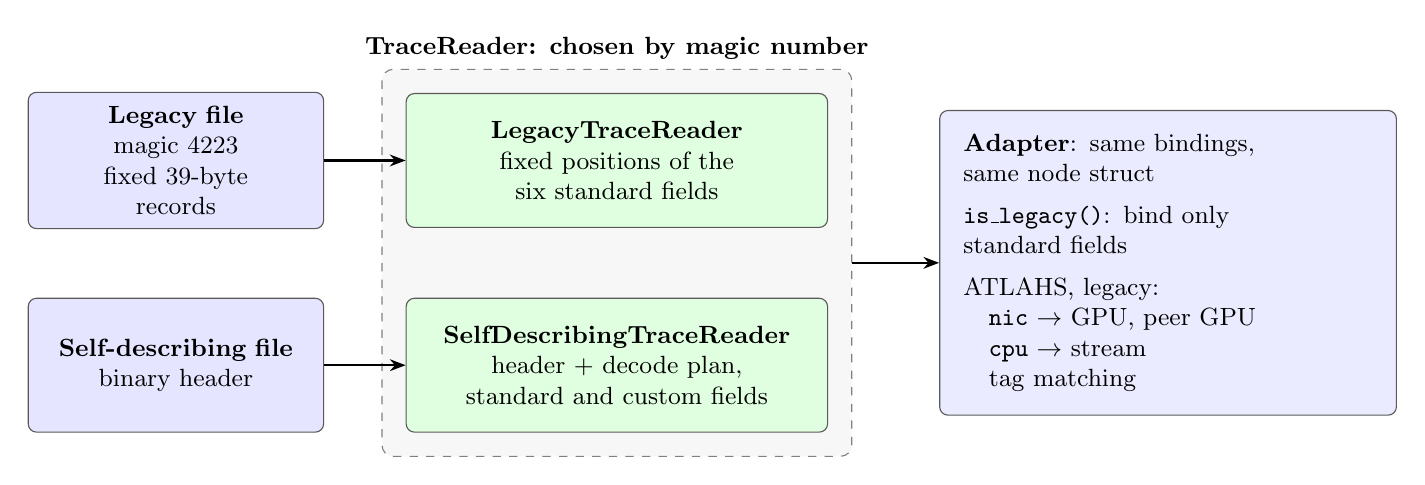
\begin{tikzpicture}[
  reader/.style={box,fill=green!12,text width=50mm,minimum height=17mm},
  file/.style={inputbox,text width=34mm,minimum height=17mm},
  adapter/.style={box,fill=blue!8,text width=52mm,align=left,inner sep=3mm}]
\node[file] (legacy) at (0,0) {\textbf{Legacy file}\\magic 4223\\fixed 39-byte\\records};
\node[file] (sd) at (0,-2.6) {\textbf{Self-describing file}\\binary header};
\node[reader] (lr) at (5.6,0) {\textbf{LegacyTraceReader}\\fixed positions of the\\six standard fields};
\node[reader] (sr) at (5.6,-2.6) {\textbf{SelfDescribingTraceReader}\\header + decode plan,\\standard and custom fields};
\draw[arrow] (legacy) -- (lr);
\draw[arrow] (sd) -- (sr);
\begin{scope}[on background layer]
  \node[draw=black!50,dashed,rounded corners=4pt,fill=black!3,inner sep=3mm,
        fit=(lr)(sr),label={[font=\small\bfseries]above:TraceReader: chosen by magic number}] (tr) {};
\end{scope}
\node[adapter] (ad) at (12.6,-1.3) {
  \textbf{Adapter}: same bindings,\\same node struct\\[4pt]
  \small\texttt{is\_legacy()}: bind only\\\small standard fields\\[4pt]
  \small ATLAHS, legacy:\\\small\quad\texttt{nic} $\rightarrow$ GPU, peer GPU\\\small\quad\texttt{cpu} $\rightarrow$ stream\\\small\quad tag matching};
\draw[arrow] (tr.east |- ad.west) -- (ad.west);
\end{tikzpicture}
}
\par\raggedright\small
\begin{itemize}
\item Existing legacy files run unchanged: the reader detects the format by its magic number.
\item The simulators have no legacy code of their own; both formats go through the same field bindings.
\item Legacy files have only the standard fields; binding a custom field to one is an error.
\item \texttt{txt2bin} still writes legacy by default; \texttt{-{}-save-mem} still invalidates the file.
\item Same output as the original LogGOPSim, with both formats, on every benchmark trace it can run.
\end{itemize}
\end{frame}


\section{Case study: ATLAHS}

\begin{frame}
\centering\vfill
{\usebeamercolor[fg]{title}\Huge\bfseries Case study: ATLAHS\par}
\vspace{4mm}
{\large Mykhaylo Gershman\par}
\vspace{3mm}
{\small\color{black!60}explicit GPU and message fields $\cdot$ scheduler fixes $\cdot$ results\par}
\vfill
\end{frame}

\begin{frame}{ATLAHS: GPU and message identity were hidden in other fields}
\vspace{6mm}
\diagram{legacy-gpu-record}
\vspace{5mm}
\begin{itemize}
\item No GPU field: the GPU goes into \texttt{nic}, the stream into \texttt{cpu}.
\item Five message-identity numbers are glued into the tag as decimal digits.
\item The file doesn't say so; htsim guesses, and a wrong guess gives wrong results without an error.
\end{itemize}
\end{frame}

\begin{frame}[fragile]{Explicit fields: eight custom fields, no format change}
\begin{lstlisting}
before: l2: send 1024b to 1 tag 3050012001 cpu 0 nic 2
after:  l2: send 1024b to 1 tag 0 cpu 0 nic 0 stream_id 0 gpu_id 2 peer_gpu_id 2
            chunk_id 3 channel_id 5 sequence_id 12 message_kind 0 communicator_id 1
\end{lstlisting}
\vspace{2mm}
\begin{itemize}
\item \textbf{Generator:} new option \texttt{-{}-explicit-fields} writes each value as a named field.
\item \textbf{New: the partner's GPU} (\texttt{peer\_gpu\_id}); the old trace had no place for it.
\item \textbf{htsim} reads both formats through our \texttt{AtlahsAdapter}; its scheduler now uses these fields (next two slides).
\end{itemize}
\end{frame}

\begin{frame}{Scheduler fix 1: messages went to the wrong GPU}
\begin{columns}[c]
\begin{column}{0.45\textwidth}
\centering
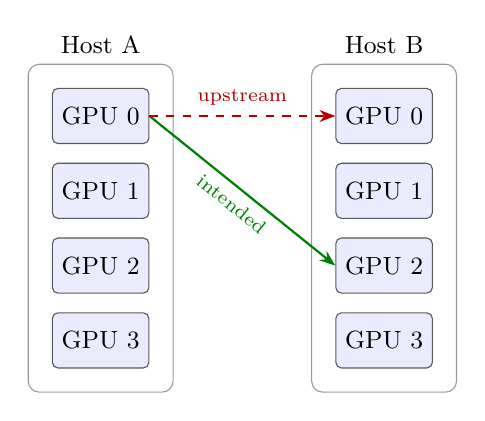
\begin{tikzpicture}[
  gpu/.style={draw=black!65,rounded corners=2pt,minimum width=9mm,minimum height=7mm,font=\small,fill=blue!8},
  host/.style={draw=black!40,rounded corners=4pt,inner sep=3mm}]
\foreach \i in {0,...,3} {
  \node[gpu] (a\i) at (0,-\i*0.95) {GPU \i};
  \node[gpu] (b\i) at (3.6,-\i*0.95) {GPU \i};
}
\node[host,fit=(a0)(a3),label=above:{\small Host A}] {};
\node[host,fit=(b0)(b3),label=above:{\small Host B}] {};
\draw[arrow,green!50!black] (a0.east) -- node[pos=0.5,below,sloped,font=\scriptsize]{intended} (b2.west);
\draw[arrow,red!70!black,dashed] (a0.east) -- node[above,font=\scriptsize]{upstream} (b0.west);
\end{tikzpicture}

\end{column}
\begin{column}{0.53\textwidth}
\small
\textbf{Problem:} upstream used the sender's GPU index at both ends. A send from A/GPU 0 to a receive on B/GPU 2 travelled to B/GPU 0, so the wrong network endpoints were simulated.
\vspace{2mm}

\textbf{Fix:} we changed htsim to send from the sender's \texttt{gpu\_id} to the receiver's \texttt{peer\_gpu\_id}. Its queues and completion callbacks now keep both endpoints, so each host updates its own resource clocks.
\vspace{2mm}

\textbf{Also:} htsim now tracks execution per \texttt{stream\_id} (32-bit) instead of the 8-bit \texttt{cpu} field; the number of streams comes from the file's schema.
\end{column}
\end{columns}
\end{frame}

\begin{frame}{Scheduler fix 2: different messages could get the same tag}
\small
Upstream, the generator glued five numbers together as decimal digits to form the tag, and htsim matched sends and receives by that one number:
\vspace{3mm}

\centering
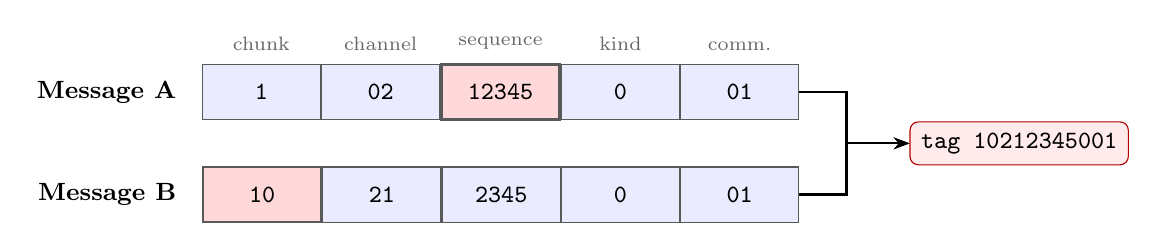
\begin{tikzpicture}[
  part/.style={draw=black!65,fill=blue!8,minimum height=7mm,minimum width=15mm,font=\small\ttfamily,inner sep=3pt},
  long/.style={part,fill=red!15,line width=0.9pt},
  lbl/.style={font=\scriptsize,text=black!60}]
\node[font=\small\bfseries,anchor=east] at (-0.2,0) {Message A};
\node[part,anchor=west] (a1) at (0,0) {1};
\node[part,right=0mm of a1] (a2) {02};
\node[long,right=0mm of a2] (a3) {12345};
\node[part,right=0mm of a3] (a4) {0};
\node[part,right=0mm of a4] (a5) {01};
\node[lbl,above=0.5mm of a1] {chunk};
\node[lbl,above=0.5mm of a2] {channel};
\node[lbl,above=0.5mm of a3] {sequence};
\node[lbl,above=0.5mm of a4] {kind};
\node[lbl,above=0.5mm of a5] {comm.};
\node[font=\small\bfseries,anchor=east] at (-0.2,-1.3) {Message B};
\node[long,anchor=west] (b1) at (0,-1.3) {10};
\node[part,right=0mm of b1] (b2) {21};
\node[part,right=0mm of b2] (b3) {2345};
\node[part,right=0mm of b3] (b4) {0};
\node[part,right=0mm of b4] (b5) {01};
\node[draw=red!70!black,fill=red!8,rounded corners=3pt,font=\small\ttfamily,inner sep=4pt,right=14mm of a5,yshift=-6.5mm] (tag) {tag 10212345001};
\draw[arrow] (a5.east) -| ([xshift=6mm]a5.east) |- (tag.west);
\draw[arrow] (b5.east) -| ([xshift=6mm]b5.east) |- (tag.west);
\end{tikzpicture}

\par\raggedright
\vspace{3mm}
\begin{itemize}
\item \textbf{Problem:} a sequence number above 9999 takes five digits instead of four and shifts the rest. Two different messages can then produce the same tag, and htsim may match a receive with the wrong send, without any error.
\item \textbf{Fix:} htsim now compares the five numbers separately, plus the sender. Explicit-field messages must use tag 0, and a message that never matches stops the run with an error.
\end{itemize}
\end{frame}

\begin{frame}{ATLAHS: a recorded Llama training run gets 54\% smaller}
\centering\vfill
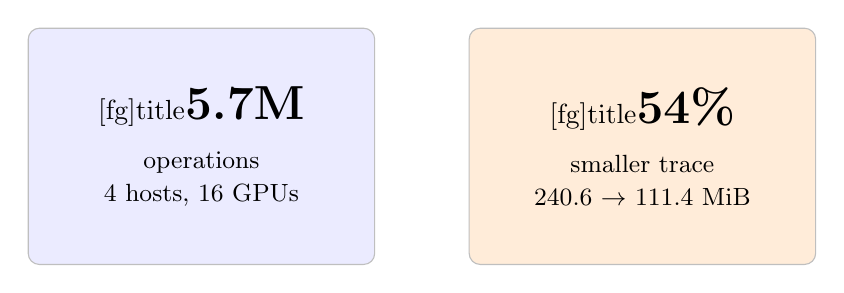
\begin{tikzpicture}
\node[card=blue!8] (c1) at (0,0) {{\usebeamercolor[fg]{title}\LARGE\bfseries 5.7M}\\[2mm]\small operations\\\small 4 hosts, 16 GPUs};
\node[card=orange!15] (c2) at (56mm,0) {{\usebeamercolor[fg]{title}\LARGE\bfseries 54\%}\\[2mm]\small smaller trace\\\small 240.6 $\to$ 111.4 MiB};
\end{tikzpicture}
\vfill
\par\raggedright
\highlight{Smaller although the new trace carries all eight ATLAHS fields.}
\end{frame}

\section{Fast decoding}

\begin{frame}
\centering\vfill
{\usebeamercolor[fg]{title}\Huge\bfseries Fast decoding\par}
\vspace{4mm}
{\large Samuel Garcin, Mykhaylo Gershman\par}
\vspace{3mm}
{\small\color{black!60}why $\cdot$ one decode plan, five runners $\cdot$ compiled and templated runners\par}
\vfill
\end{frame}

\begin{frame}{Why: decoding was up to half of the simulation time}
\centering\vfill
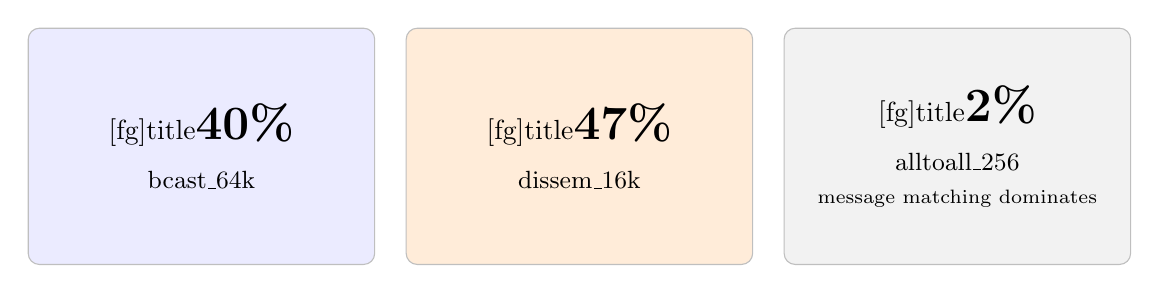
\begin{tikzpicture}
\node[card=blue!8] (c1) at (0,0) {{\usebeamercolor[fg]{title}\LARGE\bfseries 40\%}\\[2mm]\small bcast\_64k};
\node[card=orange!15] (c2) at (48mm,0) {{\usebeamercolor[fg]{title}\LARGE\bfseries 47\%}\\[2mm]\small dissem\_16k};
\node[card=black!5] (c3) at (96mm,0) {{\usebeamercolor[fg]{title}\LARGE\bfseries 2\%}\\[2mm]\small alltoall\_256\\\scriptsize message matching dominates};
\end{tikzpicture}
\vfill
\par\raggedright
\highlight{Share of the simulation time spent decoding records with the first, generic decoder, which interprets the schema for every field of every node.}
\end{frame}

\begin{frame}{One decode plan, five runners}
\vspace{3mm}
\centering\vfill
\resizebox{0.95\linewidth}{!}{% The PlanRunner interface and its implementations, in the style of schema-agreement.tex.
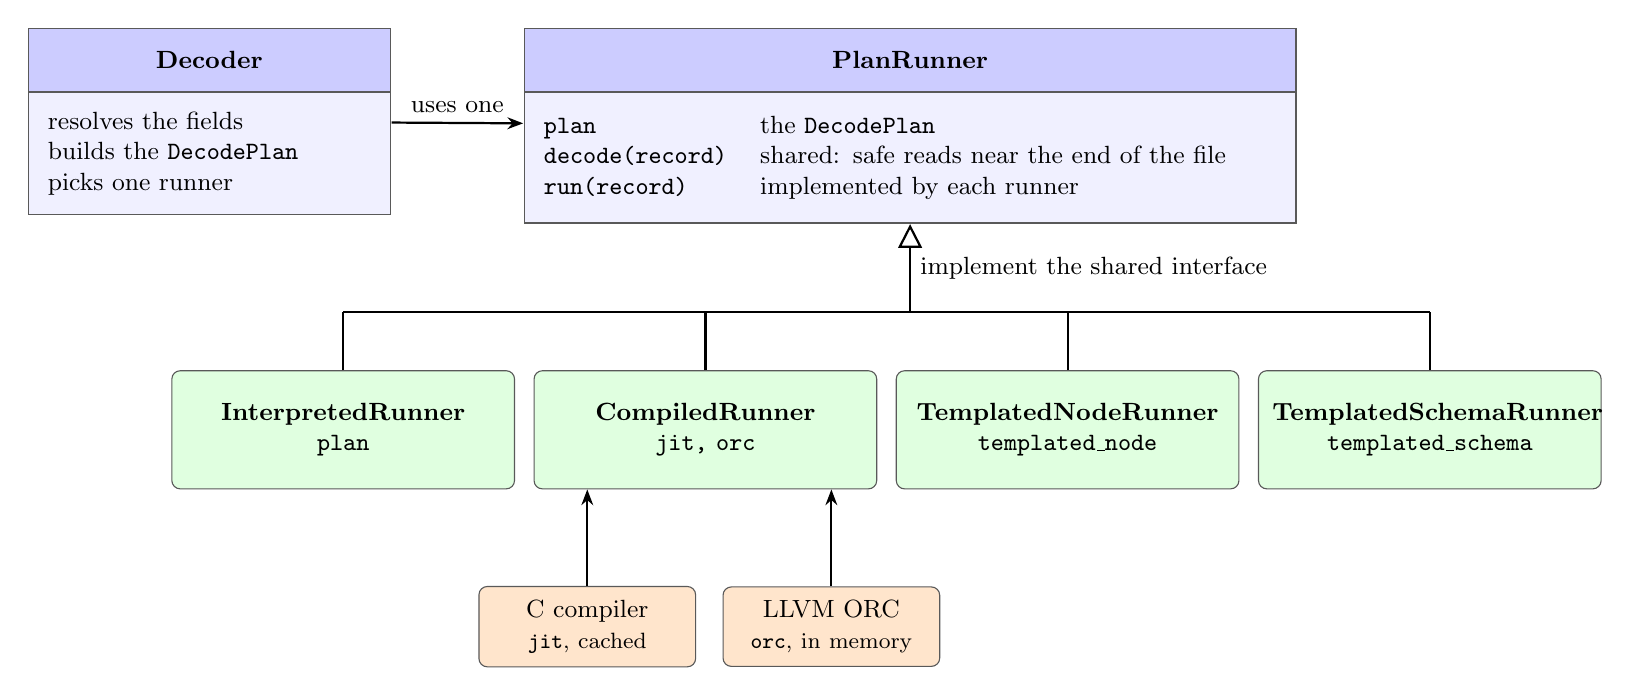
\begin{tikzpicture}[
  common/.style={box,fill=blue!8,text width=82mm,align=left,inner sep=3mm},
  runner/.style={box,fill=green!12,text width=40mm,minimum height=15mm,font=\small},
  source/.style={box,fill=orange!20,text width=24mm},
  inherits/.style={-{Triangle[open,length=3mm,width=3mm]},thick}]
% Class boxes: a header with the name, a body with one item per line.
\node[draw=black!65,fill=blue!20,minimum width=46mm,minimum height=8mm,font=\small\bfseries] (decoderhead) at (0,0.9) {Decoder};
\node[draw=black!65,fill=blue!6,text width=41mm,anchor=north,align=left,font=\small,inner sep=2.5mm] (decoderbody) at (decoderhead.south) {
  resolves the fields\\
  builds the \texttt{DecodePlan}\\
  picks one runner};
\node[fit=(decoderhead)(decoderbody),inner sep=0pt] (decoder) {};
\node[draw=black!65,fill=blue!20,minimum width=98mm,minimum height=8mm,font=\small\bfseries] (basehead) at (8.9,0.9) {PlanRunner};
\node[draw=black!65,fill=blue!6,text width=93mm,anchor=north,font=\small,inner sep=2.5mm] (basebody) at (basehead.south) {
  \begin{tabular}{@{}ll@{}}
  \texttt{plan}   & the \texttt{DecodePlan} \\
  \texttt{decode(record)} & shared: safe reads near the end of the file \\
  \texttt{run(record)}    & implemented by each runner
  \end{tabular}};
\node[fit=(basehead)(basebody),inner sep=0pt] (base) {};
\draw[arrow] (decoder) -- node[above,font=\small] {uses one} (base);
\foreach \x/\cls/\names [count=\k] in {
    1.7/InterpretedRunner/plan,
    6.3/CompiledRunner/{jit, orc},
    10.9/TemplatedNodeRunner/templated\_node,
    15.5/TemplatedSchemaRunner/templated\_schema} {
  \node[runner] (r\k) at (\x,-3.8) {\textbf{\cls}\\\texttt{\names}};
  \draw[thick] (r\k.north) -- (\x,-2.3);
}
% One inheritance arrow for all runners, as in UML.
\draw[thick] (1.7,-2.3) -- (15.5,-2.3);
\draw[inherits] (8.9,-2.3) -- node[right,font=\small] {implement the shared interface} (base.south);
\node[source] (cc) at (4.8,-6.3) {C compiler\\\footnotesize\texttt{jit}, cached};
\node[source] (llvm) at (7.9,-6.3) {LLVM ORC\\\footnotesize\texttt{orc}, in memory};
\draw[arrow] (cc.north) -- (cc.north |- r2.south);
\draw[arrow] (llvm.north) -- (llvm.north |- r2.south);
\end{tikzpicture}
}
\vfill
\end{frame}

\begin{frame}{The five runners at a glance}
\centering\vfill
\resizebox{\linewidth}{!}{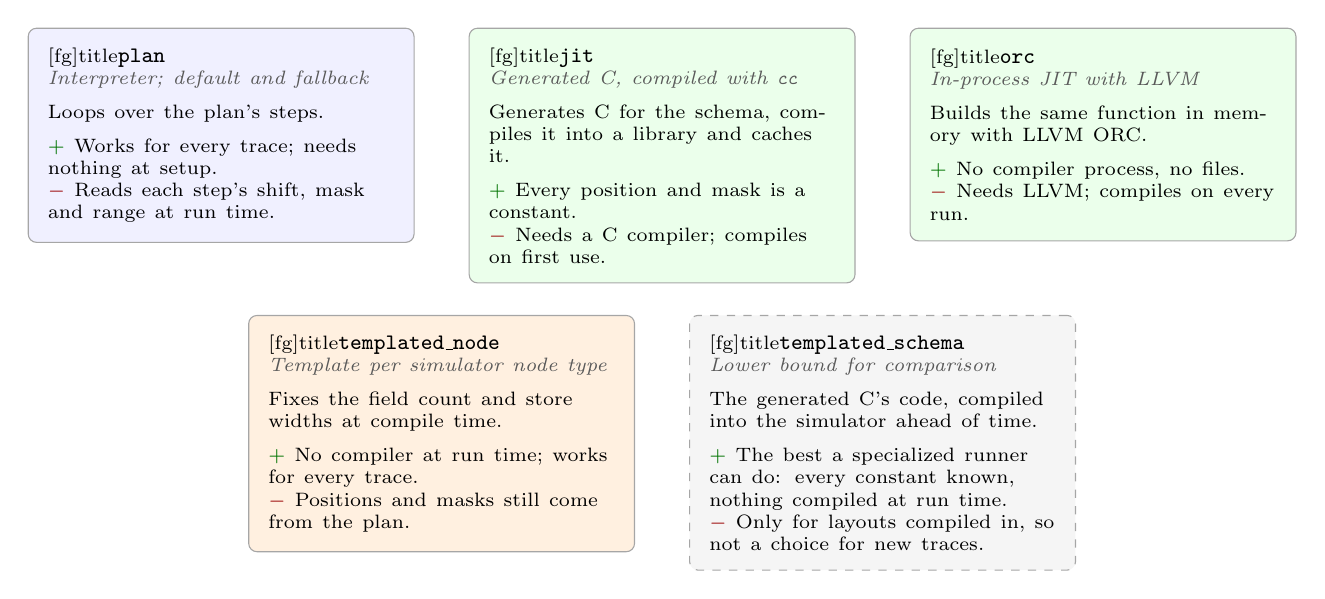
\begin{tikzpicture}
\node[runnercard=blue!6] at (0,0) {\runner{plan}{Interpreter; default and fallback}
  {Loops over the plan's steps.}
  {Works for every trace; needs nothing at setup.}
  {Reads each step's shift, mask and range at run time.}};
\node[runnercard=green!8] at (56mm,0) {\runner{jit}{Generated C, compiled with \texttt{cc}}
  {Generates C for the schema, compiles it into a library and caches it.}
  {Every position and mask is a constant.}
  {Needs a C compiler; compiles on first use.}};
\node[runnercard=green!8] at (112mm,0) {\runner{orc}{In-process JIT with LLVM}
  {Builds the same function in memory with LLVM ORC.}
  {No compiler process, no files.}
  {Needs LLVM; compiles on every run.}};
\coordinate (row2) at ([yshift=-4mm]current bounding box.south);
\coordinate (x1) at (28mm,0);
\coordinate (x2) at (84mm,0);
\node[runnercard=orange!12] at (x1 |- row2) {\runner{templated\_node}{Template per simulator node type}
  {Fixes the field count and store widths at compile time.}
  {No compiler at run time; works for every trace.}
  {Positions and masks still come from the plan.}};
\node[runnercard=black!4,dashed] at (x2 |- row2) {\runner{templated\_schema}{Lower bound for comparison}
  {The generated C's code, compiled into the simulator ahead of time.}
  {The best a specialized runner can do: every constant known, nothing compiled at run time.}
  {Only for layouts compiled in, so not a choice for new traces.}};
\end{tikzpicture}}
\vfill
\end{frame}

\begin{frame}[fragile]{Compiled runners hard-code the schema}
\begin{columns}[T]
\begin{column}{0.47\textwidth}
\begin{lstlisting}
int decode(const u8* r, u8* const* t) {
  u64 w, c;
  // type: 2 bits at bit 1, base 1
  memcpy(&w, r + 0x0, 8);
  c = (w >> 0x1) & 0x3;
  if (c > 0x2) return 0;
  c += 0x1;
  store8(t[0] + 0x38, c);
  // peer: 16 bits at bit 3
  memcpy(&w, r + 0x0, 8);
  c = (w >> 0x3) & 0xffff;
  store32(t[0] + 0x3c, c);
  // size: 0 bits, constant 1024
  store64(t[0] + 0x40, 0x400);
  // ... 8 further fields
  return 1;
}
\end{lstlisting}
\smallnote{Generated C for bcast\_64k, abridged.}
\end{column}
\begin{column}{0.5\textwidth}
\small
\begin{itemize}
\item Every position, mask and range is a constant: no loop, no dispatch; a 0-bit field is a single store.
\item \textbf{\texttt{jit}:} compiled with \texttt{cc}, cached on disk.
\item \textbf{\texttt{orc}:} the same function compiled in memory with LLVM, loaded as a plugin only when used.
\item Only numbers from the header go into the code, so a trace cannot inject code.
\end{itemize}
\end{column}
\end{columns}
\end{frame}

\section{Preliminary benchmarks}

\begin{frame}
\centering\vfill
{\usebeamercolor[fg]{title}\Huge\bfseries Preliminary benchmarks\par}
\vspace{4mm}
{\large Samuel Garcin, Mykhaylo Gershman\par}
\vspace{3mm}
{\small\color{black!60}writing: size and conversion $\cdot$ reading: throughput and startup\par}
\vspace{6mm}
\highlight{\centering One laptop (Apple M3 Pro), few repetitions. Joshua Durrant will run the full benchmarking study.}
\vfill
\end{frame}

\subsection{Writing}

\begin{frame}
\centering\vfill
{\usebeamercolor[fg]{title}\Huge\bfseries Writing\par}
\vspace{3mm}
{\large GOAL text $\to$ binary trace\par}
\vspace{3mm}
{\small\color{black!60}file size $\cdot$ conversion time\par}
\vfill
\end{frame}

\begin{frame}{Writing: file size is 26--93\% smaller}
\centering
\small
\begin{tabular}{lrrrr}
\toprule
\textbf{Trace} & \textbf{Nodes} & \textbf{Record} & \textbf{Legacy $\to$ new} & \textbf{Smaller} \\
\midrule
bcast\_8 & 14 & 39 $\to$ 2 B & 808 $\to$ 594 B & 26\% \\
bcast\_1k & 2k & 39 $\to$ 4 B & 110 $\to$ 30 KiB & 73\% \\
bcast\_64k & 131k & 39 $\to$ 4 B & 6.9 $\to$ 1.9 MiB & 73\% \\
wide\_64k (random 64-bit values) & 131k & 39 $\to$ 15 B & 6.9 $\to$ 3.2 MiB & 53\% \\
alltoall\_256 & 131k & 39 $\to$ 2 B & 5.4 MiB $\to$ 404 KiB & 93\% \\
ring\_256 & 261k & 39 $\to$ 4 B & 10.7 $\to$ 1.3 MiB & 88\% \\
dissem\_16k & 459k & 39 $\to$ 4 B & 19.2 $\to$ 2.4 MiB & 88\% \\
ATLAHS Llama run (8 extra fields) & 5.7M & 39 $\to$ 17 B & 240.6 $\to$ 111.4 MiB & 54\% \\
\bottomrule
\end{tabular}
\par\raggedright\vspace{3mm}
\begin{itemize}
\item Narrow or constant fields shrink most; even random 64-bit values save half.
\end{itemize}
\end{frame}

\begin{frame}{Writing: conversion time}
\small
Complete \texttt{txt2bin} run on the same GOAL text, \textbf{ms}.
\vspace{1mm}

\centering
\footnotesize
\begin{tabular}{lrrr}
\toprule
\textbf{Trace} & \textbf{Original \texttt{txt2bin}} & \textbf{Ours, legacy} & \textbf{Ours, new format} \\
\midrule
bcast\_8 & 53 & 51 & \textbf{3.3} \\
bcast\_1k & 63 & 119 & \textbf{7.3} \\
bcast\_64k & 758 & 4527 & \textbf{247} \\
dissem\_16k & 362 & 1462 & \textbf{333} \\
ring\_256 & \textbf{138} & 187 & 252 \\
alltoall\_256 & \textbf{74} & 136 & 82 \\
wide\_64k & 779 & 4571 & \textbf{295} \\
atlahs\_64k (8 extra fields) & n/a & n/a & 585 \\
\midrule
ATLAHS Llama run & 6\,500 & n/a & 19\,500 \\
\bottomrule
\end{tabular}
\par\raggedright\vspace{3mm}
\small
\begin{itemize}
\item New format: faster than the original on most traces despite two passes.
\item Our legacy writer remapped the file per rank (up to 6$\times$ slower); now fixed.
\end{itemize}
{\scriptsize\color{black!60}\par
Median of 5 interleaved runs. Legacy converters end with a system-wide \texttt{sync()} ($\approx$50\,ms). n/a: legacy cannot hold the custom fields (ours also rejects the Llama run's ${>}$32-bit tags). ATLAHS: one run.}
\end{frame}

\subsection{Reading}

\begin{frame}
\centering\vfill
{\usebeamercolor[fg]{title}\Huge\bfseries Reading\par}
\vspace{3mm}
{\large binary trace $\to$ simulation\par}
\vspace{3mm}
{\small\color{black!60}decoding $\cdot$ access pattern $\cdot$ startup $\cdot$ complete simulations\par}
\vfill
\end{frame}

\begin{frame}[t]{Reading: decoding throughput}
\small
Read every node once, \textbf{ns per node}; setup and compilation excluded.
\vspace{3mm}

\centering
\footnotesize
\setlength{\tabcolsep}{5pt}
\begin{tabular}{lr rrr rr}
\toprule
\textbf{Trace} & \textbf{Nodes} & \texttt{plan} & \texttt{jit} & \texttt{orc} &
\shortstack{\texttt{templated\_}\\\texttt{node}} &
\textcolor{black!55}{\shortstack{lower bound\\\texttt{(templ.\_schema)}}} \\
\midrule
bcast\_8 & 14 & 30.2 & \textbf{17.8} & \textbf{17.9} & 24.1 & \textcolor{black!55}{17.4} \\
bcast\_1k & 2k & 27.5 & \textbf{13.9} & \textbf{13.8} & 21.2 & \textcolor{black!55}{13.3} \\
bcast\_64k & 131k & 26.5 & \textbf{13.4} & \textbf{13.4} & 21.1 & \textcolor{black!55}{13.2} \\
dissem\_16k & 459k & 29.2 & \textbf{12.9} & \textbf{12.8} & 24.0 & \textcolor{black!55}{12.4} \\
ring\_256 & 261k & 30.2 & \textbf{12.7} & 13.3 & 24.0 & \textcolor{black!55}{13.1} \\
alltoall\_256 & 131k & 29.0 & \textbf{12.4} & \textbf{12.4} & 24.1 & \textcolor{black!55}{11.9} \\
wide\_64k & 131k & 26.4 & \textbf{13.7} & \textbf{13.8} & 21.1 & \textcolor{black!55}{13.5} \\
atlahs\_64k & 131k & 41.2 & 17.2 & \textbf{16.6} & 29.9 & \textcolor{black!55}{16.3} \\
\bottomrule
\end{tabular}
\par\raggedright\vspace{3mm}
\highlight{\texttt{jit} and \texttt{orc} come within 6\% of the lower bound: generated code is no longer the limit.}
{\scriptsize\color{black!60}\par\vspace{2mm}
Median of three repetitions. Bold: fastest runner (within 3\%).}
\end{frame}

\begin{frame}[t]{Reading: the simulator's access pattern}
\small
Replay of LogGOPSim's reads and counter updates, without the network model; \textbf{ns per node}.
\vspace{3mm}

\centering
\footnotesize
\setlength{\tabcolsep}{5pt}
\begin{tabular}{l r rrr rr}
\toprule
\textbf{Trace} & \textbf{Legacy} & \texttt{plan} & \texttt{jit} & \texttt{orc} &
\shortstack{\texttt{templated\_}\\\texttt{node}} &
\textcolor{black!55}{\shortstack{lower bound\\\texttt{(templ.\_schema)}}} \\
\midrule
bcast\_8 & 131 & \textbf{148} & 159 & 172 & 157 & \textcolor{black!55}{151} \\
bcast\_1k & 27.3 & 39.7 & \textbf{34.0} & \textbf{33.8} & 37.5 & \textcolor{black!55}{33.6} \\
bcast\_64k & 26.3 & 39.0 & \textbf{32.9} & \textbf{32.6} & 36.8 & \textcolor{black!55}{32.6} \\
dissem\_16k & 26.4 & 35.6 & \textbf{30.6} & \textbf{30.5} & 33.4 & \textcolor{black!55}{30.4} \\
ring\_256 & 22.6 & 36.2 & \textbf{31.7} & \textbf{31.7} & 34.3 & \textcolor{black!55}{31.3} \\
alltoall\_256 & 7.4 & \textbf{13.5} & \textbf{13.4} & \textbf{13.5} & \textbf{13.5} & \textcolor{black!55}{13.5} \\
wide\_64k & 26.1 & 39.8 & \textbf{33.7} & 35.8 & 41.1 & \textcolor{black!55}{35.7} \\
\bottomrule
\end{tabular}
\par\raggedright\vspace{3mm}
\highlight{\texttt{jit} and \texttt{orc} reach the lower bound; the remaining 4--9\,ns gap to legacy lies in record and dependency-list access, not in decoding.}
{\scriptsize\color{black!60}\par\vspace{2mm}
Median of three repetitions; bcast\_8 is dominated by fixed costs. Bold: fastest runner for the new format (within 3\%).}
\end{frame}

\begin{frame}[t]{Reading: startup cost}
\small
Setup with an \textbf{empty JIT cache}, then read every node once; no network simulation; \textbf{ms}.
\vspace{3mm}

\centering
\footnotesize
\setlength{\tabcolsep}{5pt}
\begin{tabular}{l rrr r r}
\toprule
\textbf{Trace} & \texttt{plan} & \texttt{jit} & \texttt{orc} &
\shortstack{\texttt{templated\_}\\\texttt{node}} &
\textcolor{black!55}{\shortstack{lower bound\\\texttt{(templ.\_schema)}}} \\
\midrule
bcast\_8 & \textbf{0.006} & 329 & 2.6 & \textbf{0.006} & \textcolor{black!55}{0.006} \\
bcast\_1k & 0.074 & 334 & 3.0 & \textbf{0.066} & \textcolor{black!55}{0.048} \\
bcast\_64k & 4.2 & 350 & 5.4 & \textbf{3.5} & \textcolor{black!55}{2.4} \\
dissem\_16k & 13.9 & 345 & \textbf{8.8} & 11.6 & \textcolor{black!55}{6.1} \\
ring\_256 & 8.0 & 332 & 7.3 & \textbf{7.0} & \textcolor{black!55}{3.8} \\
alltoall\_256 & 3.8 & 347 & 4.4 & \textbf{3.2} & \textcolor{black!55}{1.6} \\
wide\_64k & 4.2 & 342 & 5.7 & \textbf{3.4} & \textcolor{black!55}{2.4} \\
atlahs\_64k & 6.1 & 338 & 6.1 & \textbf{4.6} & \textcolor{black!55}{2.8} \\
\bottomrule
\end{tabular}
\par\raggedright\vspace{3mm}
\highlight{Compiling costs 330--350\,ms for \texttt{jit} and about 2.5\,ms for \texttt{orc}; \texttt{templated\_node} needs none and wins most cold starts.}
{\scriptsize\color{black!60}\par\vspace{2mm}
Median of three repetitions. Bold: fastest runner (within 3\%).}
\end{frame}

\begin{frame}[t]{Reading: complete simulations}
\vspace{-2mm}\small
Complete LogGOPSim runs including startup, \textbf{ms}; lower is better.
\vspace{1mm}

\centering
\footnotesize
\setlength{\tabcolsep}{4.5pt}
\begin{tabular}{l r r rrr r r}
\toprule
\textbf{Trace} & \shortstack{\textbf{Original}\\\textbf{LogGOPSim}} & \shortstack{\textbf{Ours,}\\\textbf{legacy}} &
\texttt{plan} & \shortstack{\texttt{jit}\\(cached)} & \texttt{orc} &
\shortstack{\texttt{templated\_}\\\texttt{node}} &
\textcolor{black!55}{\shortstack{lower bound\\\texttt{(templ.\_schema)}}} \\
\midrule
bcast\_8 & 3.1 & 3.3 & 3.3 & 3.6 & 12.8 & 3.4 & \textcolor{black!55}{3.2} \\
bcast\_1k & 3.8 & 3.9 & 3.9 & 4.1 & 13.2 & 3.9 & \textcolor{black!55}{3.8} \\
bcast\_64k & 48.4 & 43.9 & 45.1 & 43.7 & 52.9 & 44.1 & \textcolor{black!55}{43.6} \\
dissem\_16k & 146.4 & 122.7 & 116.6 & 110.8 & 118.3 & 114.3 & \textcolor{black!55}{110.2} \\
ring\_256 & 39.8 & 32.8 & 34.5 & 32.9 & 41.8 & 33.6 & \textcolor{black!55}{32.4} \\
alltoall\_256 & 1950 & 2004 & 1997 & 1996 & 2010 & 1999 & \textcolor{black!55}{1998} \\
wide\_64k & crashes & 78.4 & 79.6 & 79.5 & 88.3 & 81.3 & \textcolor{black!55}{77.8} \\
\bottomrule
\end{tabular}
\par\raggedright\vspace{1mm}
\small
\begin{itemize}\setlength{\itemsep}{0pt}
\item Larger collectives: all runners but \texttt{orc} (loads LLVM in every run) are 7--24\% faster than the original.
\item alltoall\_256: message matching dominates, at most 3\% slower. Results identical everywhere; the original crashes on wide\_64k.
\end{itemize}
{\scriptsize\color{black!60}\par
Median of 21 runs, configurations interleaved in a seeded random order. Original: last upstream commit (76451de), same build type, on the legacy files.}
\end{frame}

\begin{frame}{Which runner wins where}
\centering
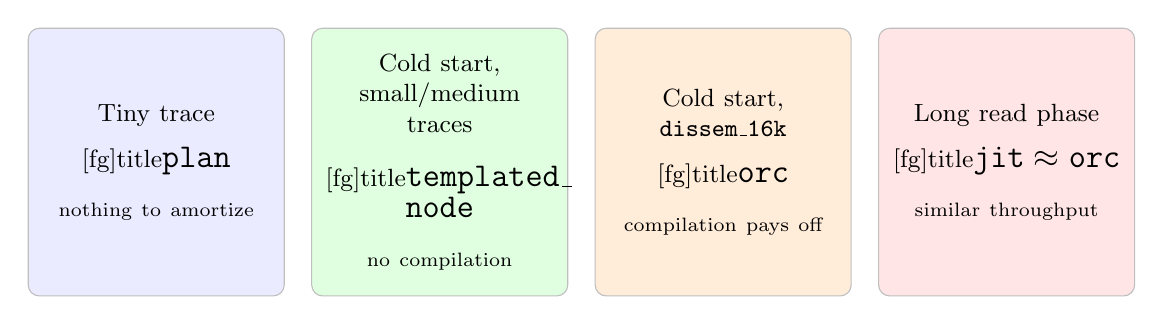
\begin{tikzpicture}[choice/.style={text width=29mm,minimum width=0pt,minimum height=34mm}]
\node[card=blue!8,choice] at (0,0) {\small Tiny trace\\[2mm]{\usebeamercolor[fg]{title}\large\bfseries\texttt{plan}}\\[2mm]\scriptsize nothing to amortize};
\node[card=green!12,choice] at (36mm,0) {\small Cold start,\\small/medium traces\\[2mm]{\usebeamercolor[fg]{title}\large\bfseries\texttt{templated\_}\\\texttt{node}}\\[2mm]\scriptsize no compilation};
\node[card=orange!15,choice] at (72mm,0) {\small Cold start,\\\texttt{dissem\_16k}\\[2mm]{\usebeamercolor[fg]{title}\large\bfseries\texttt{orc}}\\[2mm]\scriptsize compilation pays off};
\node[card=red!10,choice] at (108mm,0) {\small Long read phase\\[2mm]{\usebeamercolor[fg]{title}\large\bfseries\texttt{jit} $\approx$ \texttt{orc}}\\[2mm]\scriptsize similar throughput};
\end{tikzpicture}
\par\raggedright\vspace{5mm}
\small
\begin{itemize}
\item Lower bound (\texttt{templated\_schema}): after setup, \texttt{jit} and \texttt{orc} come within 6\% of it; at startup, the best runner needs 1.4--2$\times$ its time.
\item Measured on one laptop; automatic selection needs crossover points on more layouts.
\end{itemize}
\end{frame}

\section{Next steps}

\begin{frame}{Next steps}
\begin{columns}[T]
\begin{column}{0.49\textwidth}
\small
\textbf{Reading}
\begin{itemize}
\item Select the runner using startup cost, trace size and cache availability.
\item Profile the remaining rank-lookup, packed-index and counter-update costs.
\end{itemize}
\vspace{3mm}
\textbf{Writing}
\begin{itemize}
\item Make legacy I/O comparable: per-rank remapping and flush policy.
\item Measure the phases, then evaluate a lean analysis pass or dictionary encoding.
\end{itemize}
\end{column}
\begin{column}{0.47\textwidth}
\small
\textbf{Evaluation}
\begin{itemize}
\item Euler study (Joshua): Linux/x86-64, cold file caches and peak memory.
\item Larger recorded workloads and custom-field-heavy traces.
\item Parallelization (Alexander): pass 2 and the legacy writer, keeping cross-format and cross-runner checks.
\end{itemize}
\end{column}
\end{columns}
\end{frame}

\section{Questions}

\begin{frame}{Questions}
\begin{itemize}
\item \textbf{Runner selection:} should cold-start cost or repeated-read throughput guide the default? Keep an explicit override?
\vspace{4mm}
\item \textbf{Writing:} after matching I/O policies, should we prioritize a cheaper analysis pass or dictionary compression?
\vspace{4mm}
\item \textbf{Evaluation:} which larger workloads and cold-cache scenarios should the Euler study prioritize?
\end{itemize}
\end{frame}

\end{document}
